\documentclass[a4paper, 12pt, openany, oneside, brazil]{abntex2} %\usepackage[latin1]{inputenc}
\usepackage[utf8]{inputenc}
\usepackage[brazil]{babel}
\usepackage[T1]{fontenc}
\usepackage{graphicx}
\usepackage{indentfirst}
\usepackage{listings}  % Para implementar códigos dentro do arquivo
\usepackage{color}     % Color
\usepackage{amsmath}
\usepackage{amssymb}  % simbolo logo \therefore
\usepackage{cancel}
% \usepackage{subcaption}
\usepackage[T1]{fontenc}		% Selecao de codigos de fonte.
\usepackage[brazilian,hyperpageref]{backref}	 % Paginas com as citações na bibl
\usepackage[num, bibjustif]{abntex2cite}	% Citações padrão ABNT

\usepackage{lmodern}			% Usa a fonte Latin Modern
\DeclareUnicodeCharacter{00A0}{ }

% define the author
\autor{David Oliveira da Fonseca e Marcus Vinícius Araújo Moreno.}
\titulo{Análise de uma turbina hidráulica em um modelo reduzido}
\instituicao{Universidade Federal do Rio de Janeiro - UFRJ}
\local{Macaé/RJ}
\data{2015}
\instituicao{Universidade Federal do Rio de Janeiro - \textit{campus} Macaé}

\tipotrabalho{Trabalho Acadêmico}

\preambulo{Projeto semestral para aprovação da disciplina de Projetos de Escoamento, ministrado pelo Prof. Eng. Marcelo Silva da Universidade Federal do Rio de Janeiro - \textit{campus} Macaé.}

\makeatletter
\hypersetup{
        %pagebackref=true,
		pdftitle={\@title},
		pdfauthor={\@author},
    	pdfsubject={\imprimirpreambulo},
	    pdfcreator={LaTeX with abnTeX2},
		pdfkeywords={abnt}{latex}{abntex}{abntex2}{relatório técnico},
		colorlinks=true,       		% false: boxed links; true: colored links
        % colorlinks=false,
    	linkcolor=blue,          	% color of internal links
    	citecolor=blue,        		% color of links to bibliography
    	filecolor=magenta,      		% color of file links
		urlcolor=blue,
		bookmarksdepth=4
}
\makeatother

% ---
% Espaçamentos entre linhas e parágrafos
% ---

% O tamanho do parágrafo é dado por:
\setlength{\parindent}{1.3cm}

% Controle do espaçamento entre um parágrafo e outro:
\setlength{\parskip}{0.2cm}  % tente também \onelineskip
% ---
% compila o indice
% ---
\makeindex
% ---

\newcommand*\rfrac[2]{{}^{#1}\!/_{#2}}
\renewcommand{\arraystretch}{1.3}
\newcommand{\volume}{\mathop{\ooalign{\hfil$V$\hfil\cr\kern0.08em--\hfil\cr}}\nolimits}

\definecolor{codegreen}{rgb}{0,0.6,0}
\definecolor{codegray}{rgb}{0.5,0.5,0.5}
\definecolor{codepurple}{rgb}{0.58,0,0.82}
\definecolor{backcolour}{rgb}{0.95,0.95,0.92}

\lstdefinestyle{mystyle}{
    backgroundcolor=\color{backcolour},
    commentstyle=\color{codegreen},
    keywordstyle=\color{magenta},
    numberstyle=\tiny\color{codegray},
    stringstyle=\color{codepurple},
    basicstyle=\footnotesize,
    breakatwhitespace=false,
    breaklines=true,
    captionpos=b,
    keepspaces=true,
    numbers=left,
    numbersep=5pt,
    showspaces=false,
    showstringspaces=false,
    showtabs=false,
    tabsize=2
}
\lstset{style=mystyle}

\begin{document}

\frenchspacing

\imprimircapa

\imprimirfolhaderosto

% ---
% RESUMOS
% ---

% resumo em português
\setlength{\absparsep}{18pt} % ajusta o espaçamento dos parágrafos do resumo
\begin{resumo}

    O trabalho a seguir foi elaborado para consolidar e concatenar o conteúdo aprendido no eixo de disciplinas Sistema de Escoamentos da UFRJ - \textit{campus} Macaé. Seu objetivo compreender os fundamentos teóricos necessários para a construção de um modelo reduzido para uma turbina hidráulica. Para isso, foi necessário avaliar a perda de carga em uma tubulação, bem como os cálculos do modelo reduzido. A metodologia baseou-se em encontros quinzenais com o Prof. Eng. Marcelo Silva que orientou a conclusão deste trabalho. Conclui-se que 

 \textbf{Palavras-chaves}: turbina hidráulica. modelo reduzido. perda de carga.

\end{resumo}

% resumo em inglês
\begin{resumo}[Abstract]
 \begin{otherlanguage*}{english}
   This is the english abstract.

   \vspace{\onelineskip}

   \noindent
   \textbf{Key-words}: latex. abntex. text editoration.
 \end{otherlanguage*}
\end{resumo}

% ---
% inserir o sumario
% ---
\pdfbookmark[0]{\contentsname}{toc}
\tableofcontents
\cleardoublepage
% ---

% ----------------------------------------------------------
% ELEMENTOS TEXTUAIS
% ----------------------------------------------------------
\textual

% ---
% Trabalho tod
% ---
\OnehalfSpacing

\chapter*[Objetivo]{Objetivo}
\addcontentsline{toc}{chapter}{Objetivo}
    Este trabalho pretende demonstrar habilidade na elaboração de um trabalho acadêmico, além do domínio adquirido pelo grupo na análise de modelo reduzido assim como avaliação da perda de carga de uma tubulação, assimilados no decorrer das disciplinas de Mecânica dos Fluidos e Máquinas de Fluxo I. Nele, encontra-se a apresentação do problema proposto com seus respectivos cálculos e comentários sobre os resultados.

    Deseja-se construir um modelo de dimensões 10 (dez) vezes menores, submetido a uma altura de queda também 10 (dez) vezes menor para uma turbina hidráulica que opera com água. De modo que pode-se prever o funcionamento da turbina, como a velocidade de rotação, a potência no eixo e o diâmetro do rotor.


\chapter{Fundamentos Teóricos}
% % \chapter*[Introdução]{Introdução}
% \addcontentsline{toc}{chapter}{Introdução}

% \chapter{Fundamentos Teóricos}

\section{Máquinas de fluxo}

	Máquinas de fluxo são caracterizadas por ser um transformador de energia, em que necessariamente uma das formas de energia é o trabalho mecânico, e a outra é energia de fluido \cite{maq_fluidos_henn}. Quando esse fluido passa por um elemento rotativo, ocorre a transformação de energias. Se a máquina de fluxo recebe trabalho mecânico e o transforma em energia de fluido, chamamos de máquinas de fluxo geradora, pois a energia do fluido aumenta. Desse tipo, são caracterizados as bombas centrífugas e ventiladores. Se a máquina de fluxo recebe energia de fluido e o transforma em trabalho mecânico, chamamos de máquinas de fluxo motora. Desse tipo, são exemplos as turbinas hidráulicas e turbinas a vapor, que será o foco desse trabalho.

\subsection{Elementos fundamentais da máquina de fluxo}

    Para cada máquina de fluxo, existem diversos elementos que a compõem e não será tratado aqui todos eles, mas sim os fundamentais para o funcionamento da máquina. Como o rotor (elemento rotativo) e o sistema diretor.

	Rotor é o elemento rotativo principal de uma máquina de fluxo, é onde ocorre a transformação de energia mecânica em energia de fluido ou vice-versa. É composto por um certo número de pás giratórias que dividem o espaço ocupado em canais, por onde circula o fluido de trabalho, conforme mostrado na \autoref{fig1:rotor_bomba}.

    \begin{figure}[htb]
        \centering
        \caption {\label {fig1:rotor_bomba} Rotor de uma bomba fluxo semi-axial ou fluxo misto}
        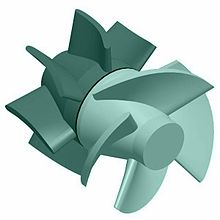
\includegraphics[scale=0.65]{images/fig1.png}
        \legend{Fonte: Wikipédia \cite{wiki_bomba_axial}}
        % \legend{Fonte: Wikipédia \footnote{Bombas Axiais}}
    \end{figure}


    Já o sistema diretor, tem como função, coletar o fluido e dirigi-lo para um caminho determinado. No caso das bombas centrífugas, o sistema diretor de saída é simplesmente um difusor, que transforma parte da energia de velocidade em energia de pressão. Já nas turbinas, o sistema diretor é fundamentalmente um injetor, conforma mostrado na \autoref{fig2:sist_diretor_pelton}, que transforma parte da energia de pressão em energia de velocidade.

    \begin{figure}[htb]
        \centering
        \caption {\label {fig2:sist_diretor_pelton} Sistema diretor de uma turbina hidráulica do tipo Pelton}
        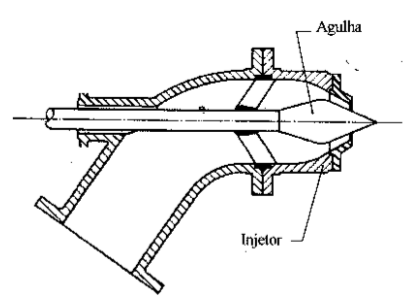
\includegraphics[scale=0.5]{images/fig2.png}
        \legend{Fonte: Máquinas de Fluidos \cite{maq_fluidos_henn}}
    \end{figure}

\subsection{Tipos de Turbinas Hidráulicas}

\subsubsection{Turbina tipo Francis}

A turbina Francis, é uma turbina hidráulica que foi concebida por Jean-Victor Poncelet por volta de 1820 e aperfeiçoado pelo engenheiro norte-americano James B. Francis \cite{turbina_francis}. Ela se comporta com o fluxo radial de fora para dentro, conforme pode ser visto na Figura \ref{fig3:turbina_francis}.

    \begin{figure}[htb]
        \centering
        \caption {\label{fig3:turbina_francis} Ilustração de uma turbina Francis}
        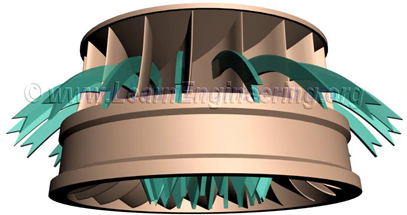
\includegraphics[scale=0.8]{images/fig3.png}
        \legend{Fonte: Learn Engineering \cite{francis_turbine}}
    \end{figure}

    É uma das turbinas mais utilizadas na produção de energia elétrica devido ao seu alto grau de eficiência em um grande ramo de operações. O \textit{head} pode variar de 45 a 400 m, e a vazão de 10 a 700 $m^3/s$. \cite{francis_turbine}

\subsubsection{Turbina tipo Kaplan}

    A turbina Kaplan é uma turbina hidráulica, inventada por Victor Kaplan. Foi uma evolução da turbina Francis para ter um melhor rendimento com quedas menores. Ela foi projetada para operar com quedas até de 60m, normalmente utilizada entre 2 a 25 e com alta vazão, entre 70 a 800 $m^3/s$. A única diferença entre a turbina Kaplan e a Francis, é o rotor. O rotor da Kaplan se assemelha a um propulsor de navio, conforme pode ser visto na  \autoref{fig4:turbina_kaplan}.

    \begin{figure}[htb]
        \centering
        \caption {\label {fig4:turbina_kaplan} Turbina Kaplan depois de 61 anos de uso. }
        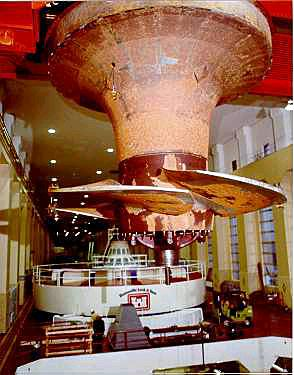
\includegraphics[scale=0.6]{images/fig4.jpg}
        \legend{Fonte: Wikipedia \cite{turbina_kaplan}}
    \end{figure}

\subsubsection{Turbina tipo Pelton}

    \begin{figure}[htb]
        \centering
        \caption {\label{fig5:turbina_pelton} Funcionamento da turbina Pelton}
        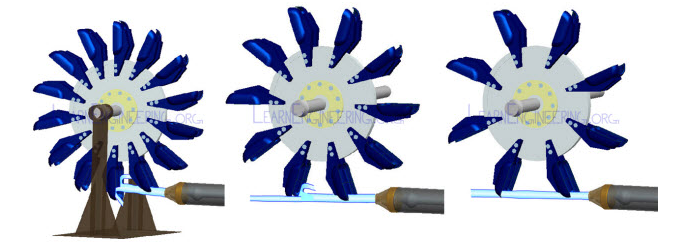
\includegraphics[scale=0.5]{images/fig5.png}
        \legend{Fonte: Learn Engineering \cite{pelton_turbine}.}
    \end{figure}

    Turbina Pelton é uma turbina de ação, isto é, funciona à pressão atmosférica, são adequadas para alto \textit{head}, variando entre 350 $m$ até 1100 $m$ e baixa vazão \cite{pelton_turbine}. Foi inventada por Lester Allan Pelton na década de 1870 \cite{turbina_pelton}.

    É constituída por uma roda, com um ou mais injectores e pás giratórias em forma de dupla concha conforme pode ser visto na \autoref{fig5:turbina_pelton}. Basicamente a turbina Pelton transforma a energia de pressão proveniente do jato de água em alta velocidade em energia de cinética, pois quando o jato incide na dupla concha da turbina Pelton, produz uma força impulsiva que a turbina se movimenta. O eixo rotativo executa um gerador que produz eletricidade.

\subsection{Campo de Aplicação}

    \begin{figure}[htb]
        \centering
        \caption{\label{fig-camp} Campo de aplicação}
        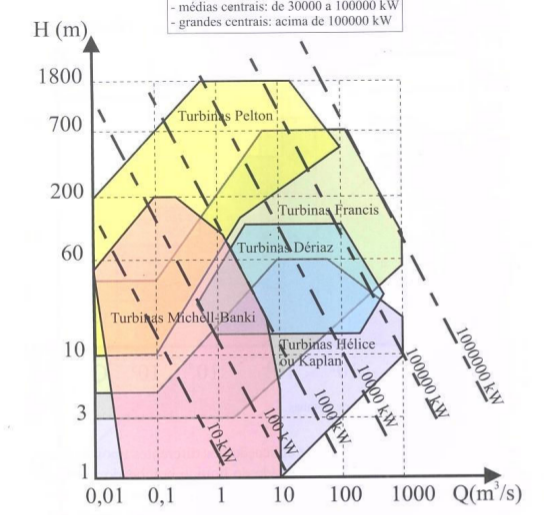
\includegraphics[scale=0.5]{images/campo_de_aplicacao.png}
        \legend{Fonte: Máquinas de Fluidos  \cite{maq_fluidos_henn}.}
    \end{figure}

    Para o ramo das turbinas, existem áreas de superposição entre os campos de aplicação dos diferentes tipos de turbinas, levando em consideração a altura de queda, vazão e a potência. A \autoref{fig-camp} releva predominância em certas áreas de aplicação, como por exemplo de elevada altura de queda e baixa vazão, a turbina Pelton se destaca. Enquanto para grandes vazões e pequena altura de queda a Kaplan se destaca.

\section{Triangulo de Velocidades}

    Um dos conceitos-chave em máquinas de fluxo é entender como o escoamento aparece do ponto de visto do elemento rotativo. Uma vez entendido isso, o entendimento da máquinas de fluxo se torna relativamente mais fácil. Observar a velocidade do escoamento a partir do ponto de vista do rotor em movimento é chamado de \textit{velocidade relativa da corrente fluida} ($\vec{w}$) e a velocidade do escoamento do ponto de vista do observador estacionário é chamado de \textit{velocidade absoluta da corrente fluida} ($\vec{c}$).


    % \begin{figure}[htb]
    %     \centering
    %     \caption {\label{fig7:2motion} Triângulo de velocidades (analogia com o movimento das partículas de água da chuva)}
    %     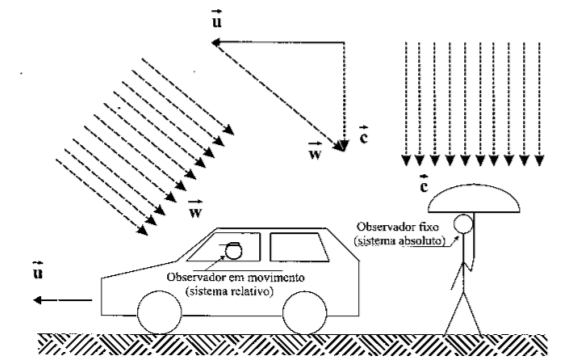
\includegraphics[scale=0.6]{images/fig7.png}
    %     \legend{Fonte: Máquinas de Fluidos  \cite{maq_fluidos_henn}.}
    % \end{figure}
    %
    % Na \autoref{fig7:2motion}, observa-se soma vetorial para o triangulo de velocidades da água da chuva com um carro em movimento, portanto se o observador está em  movimento (como é o caso do elemento rotativo nas máquinas de fluxo), com velocidade $\vec{u}$ e a chuva com a velocidade absoluta da corrente fluida $\vec{c}$, e a soma vetorial dessas velocidades será a velocidade relativa da corrente fluida $\vec{w}$ em relação ao observador em movimento.
    %
    % Nas máquinas de fluxo, o triangulo de velocidades ocorre de forma semelhante conforme demostrado acima. 
    A \autoref{fig8:tri_vel} representa o corte segundo um plano meridiano que passa pelo eixo do rotor e pelo corte segundo um plano perpendicular ao eixo do rotor de uma corrente fluida que circula através do rotor de um ventilador (máquina geradora de fluxo).

    \noindent
    Em um ponto qualquer do rotor, denomina-se: \\
        $\vec{u}$ = \textbf{velocidade tangencial} do referido ponto do rotor; \\
        $\vec{c}$ = \textbf{velocidade absoluta da corrente fluida}; \\
        $\vec{w}$ = \textbf{velocidade relativa da corrente fluida}; \\
        $\alpha$ = ângulo que formam os sentidos positivos de $\vec{u}$ e $\vec{c}$ ; \\
        $\beta$ = ângulo que formam o sentido de $\vec{w}$ com o negativo de $\vec{u}$

    \begin{figure}[htb]
        \centering
        \caption {\label{fig8:tri_vel} Escoamento através do rotor de um ventilador centrífugo (máquina de fluxo geradora)}
        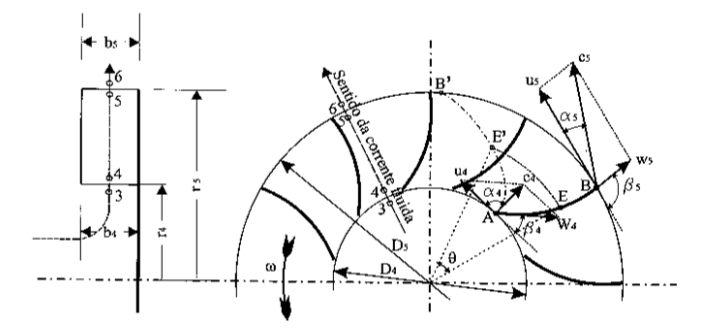
\includegraphics[scale=0.65]{images/fig8.png}
        \legend{Fonte: Máquinas de Fluidos  \cite{maq_fluidos_henn}.}
    \end{figure}

    \noindent
        A estes vetores e suas componentes atribuem-se os seguintes índices: \\
        \textbf{3} = um ponto na corrente de entrada não perturbada, situado imediatamente antes da \textbf{entrada} do rotor; \\
        \textbf{4} = um ponto situado imediatamente depois da entrada do rotor, portanto, já no espaço entre as pás giratórias; \\
        \textbf{5} = um ponto situado imediatamente antes da \textbf{saída} do rotor, portanto, ainda no espaço entre as pás giratórias; \\
        \textbf{6} = um ponto  na corrente de saída não perturbada, situado imediatamente depois da saída do canal móvel.

        Considere a \autoref{fig8:tri_vel} um rotor radial constituído de um número infinito de pás, de espessura infinitesimal, separadas por canais infinitesimais também. Isso implica que o fluxo através dele será unidimensional e que a corrente fluida será tangente às pás do rotor, em todos os seus pontos.

        As pás são construídas de modo inicial para que não haja mudança brusca de direção e perdas de energias devido a formação de vórtices por exemplo. No ponto \textit{A} temos o triângulo de velocidades da corrente fluida imediatamente após a entrada do rotor, e no ponto \textit{B} o triângulo de velocidades da corrente fluida imediatamente antes da saída do rotor. A \autoref{fig9:tri_vel} representa um triângulo de velocidades genérico, em que se faz a decomposição dos vetores $\vec{c}$ e $\vec{w}$ em componentes meridianas com o índice \textit{m} e em componentes tangenciais com o índice \textit{u}.

    \begin{figure}[htb]
        \centering
        \caption {\label {fig9:tri_vel} Triangulo de velocidades genérico }
        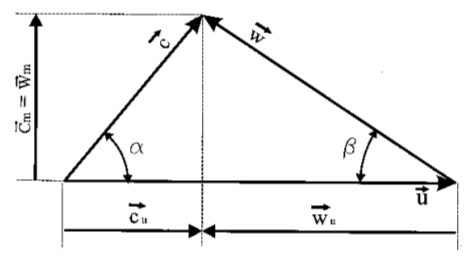
\includegraphics[scale=0.65]{images/fig9.png}
        \legend{Fonte: Máquinas de fluidos  \cite{maq_fluidos_henn}}
    \end{figure}

    A componente tangencial está vinculada com a energia intercambiada entre o rotor e o fluido, enquanto a componente meridiana, de módulo $\vec{c}_m$ está vinculada à vazão da máquina, por meio da equação da continuidade: Q = A $c_m$.

% \section{Máquinas Semelhantes}
%
% \chapter{Motivação}
%
% \section{Exemplos de modelo reduzido}
%
% \section{Projeto}
%
% \chapter{Cálculo e Explicações}

% \chapter*[Considerações Finais]{Considerações Finais}
% \addcontentsline{toc}{chapter}{Considerações Finais}

% \section {Números adimensionais}

\subsection{Coeficiente de Reynolds}

    O número de Reynolds é bastante utilizado na mecânica dos fluidos, principalmente para determinar a classificação do escoamento, se é laminar, transiente ou turbulento. Seu significado físico é o quociente de forças de inércia ($V \rho$) entre forças de viscosidade ($\mu/D$), e é expressado como:

    \begin{equation} \label{eq-reynolds}
        Re = \frac{\rho V D}{\mu}
    \end{equation}

    Onde, $\rho$ é a massa específica do fluido, $V$ velocidade do fluido, $D$ o diâmetro da tubulação e $\mu$ a viscosidade cinemática do fluido.

\subsection {Coeficiente de forma}

    A equação abaixo representa a \textbf{velocidade de rotação específica} ou \textbf{coeficiente de forma} do rotor. Ela é adimensional e seu valor numérico mantém constante para máquinas de fluxo semelhantes, independente do sistema de unidades usado no cálculo.
    \begin{equation} \label{eq-na}
        n_{qA} = 10^3 \; . \; n \; . \; \frac{Q^{\rfrac{1}{2}}}{Y^{\rfrac{3}{4}}}
    \end{equation}

\noindent
    Onde:  \\
    $n_{qA} =$ velocidade de rotação específica ou coeficiente de forma do rotor; \\
    $n$ = velocidade de rotação da máquina, em $rps$ (Hz); \\
    $Q$ = vazão da máquina, em $m^3/s$; \\
    $Y$ = salto energético específico, em $J/kg$.

% \indent

    Os valores de $n$, $Q$, e $Y$, utilizados no cálculo do $n_{qA}$ correspondem ao ponto de projeto ou melhor rendimento. Para máquinas de vários estágios (rotores em série) o $Y$ utilizado corresponde ao salto energético específico de cada rotor, e para rotores com dupla sucção, utiliza-se a vazão $Q$ de um dos tubos de sucção.

    \begin{table}[htb]
         \setlength{\tabcolsep}{20pt} % General space between cols (6pt standard)
        \centering
        \caption{Valores de $n_{qA}$ indicados para diferentes tipos de máquinas de fluido.}
        \label{tab-na}
        % \begin{tabular}{p{2.6cm}|p{6.0cm}|p{2.25cm}|p{3.40cm}}
        % \resizebox{0.35\textwidth}{!}{%
        \begin{tabular}{l  l}
            \toprule
            Para turbina hidráulica do tipo Pelton & $n_{qA} =$ 5 a 70 \\
            \hline
            Para turbina hidráulica do tipo Francis lenta & $n_{qA} =$ 50 a 120 \\
            % \hline
            % Para turbina hidráulica do tipo Francis normal & $n_{qA} =$ 120 a 200 \\
            \hline
            Para turbina hidráulica do tipo Francis rápida & $n_{qA} =$ 200 a 320 \\
            \hline
            Para turbina hidráulica do tipo Michel-Banki  & $n_{qA} =$ 30 a 210 \\
            \hline
            Para turbina hidráulica do tipo Dériaz  & $n_{qA} =$ 200 a 450 \\
            \hline
            Para turbina hidráulica do tipo Kaplan e Hélice  & $n_{qA} =$ 300 a 1000 \\
            \hline
            Para turbina a vapor e gás com admissão parcial & $n_{qA} =$ 6 a 30 \\
            \hline
            Para turbina a vapor e gás com admissão total & $n_{qA} =$ 30 a 300 \\
            \hline
            Para bomba de deslocamento positivo & $n_{qA} <$  30 \\
            \hline
            Para bomba centrifuga & $n_{qA} =$  30 a 250 \\
            \hline
            Para compressor de deslocamento positivo & $n_{qA} <$ 20 \\
            \hline
            Para ventilador e turbocompressor centrífugo & $n_{qA} = 20$ a 330 \\
            \hline
            Para ventilador e turbocompressor axial & $n_{qA} =$ 330 a 1800 \\
            \bottomrule
        \end{tabular} %}
        \legend {Fonte: Máquinas de fluidos  \cite{maq_fluidos_henn}}
    \end{table}


\section{Perda de Carga}

    O assunto perda de carga é extenso dentro da mecânica dos fluidos, será tratado aqui apenas o essencial para o desenvolvimento do projeto. Sabe-se que entre dois pontos de um fluido é possível aplicar a equação abaixo, com as seguintes condições: escoamento permamente, incompreensível, completamente desenvolvido, energia interna e pressão uniforme em 1 e 2 \cite{fox}.

    \begin{equation} \label{eq-perda_de_carga}
        h_t = \left( \frac{p_1}{\rho} + \frac{V^2_1}{2} + gz_1 \right)- \left( \frac{p_2}{\rho} + \frac{V^2_2}{2} + gz_2 \right)
    \end{equation}

\noindent
    Onde: \\
    $h_t$ : Perda de carga total da tubulação entre os pontos 1 e 2. \\
    $p$   : Pressão nos pontos 1 e 2. \\
    $\rho$ : Massa específica do fluido. \\
    $z$ : Cota geométrica do ponto 1 e 2. \\
    $V$: Velocidade nos pontos 1 e 2.


    Para um escoamento laminar, é possível calcular a ($h_t$) analiticamente, porém tubulação desenvolvida para o projeto, o escoamento é turbulento e o cálculo da perda de carga ($h_t$) é encontrado por uma fórmula empírica em base dados experimentais, conhecida por Darcy-Weisbach:
    \begin{equation} \label{eq-darcy}
        h_{maior} = f \frac{L}{D} \frac{V^2}{2}
    \end{equation}

    \noindent
    Onde \\
    $f$: fator de atrito \\
    $L$: Comprimento do duto \\
    $D$: Diâmetro interno do duto \\
    $V$: Velocidade no duto

    E $h_{maior}$ é denominado perda de carga maior, pois é onde terá uma maior contribuição para a perda de carga total, as perdas menores são devido uma variedade de acessórios, curvas ou mudanças súbitas de área \cite{fox} que não serão consideradas na tubulação do projeto.

    O fator de atrito $f$ pode ser calculado através da fórmula de Colebrook \cite{fox}, que serve para evitar o uso do Diagrama de Moody nos escoamentos turbulentos:

    \begin{equation} \label{eq-colebrook}
    \frac{1}{f^{0,5}} = -2,0 \log \left( \frac{e/D}{3,7} + \frac{2,51}{Re\;f^{0,5}} \right)
    \end{equation}

    Que é facilmente resolvida dando-lhe um valor inicial arbitrário  e fazendo a iteração dos novos valores, pois converge rapidamente.

\section{Máquinas de fluxo semelhantes}

    Há diversas vantagens em se construir máquinas de fluxo semelhantes, enquanto para modelos reduzidos permite diminuir a execução errônea de máquinas de grande porte, a construção de modelos aumentados muitas vezes se faz necessária para facilitar as medições durante os ensaios \cite{maq_fluidos_henn}.

    Para que duas máquinas sejam consideradas semelhantes, é necessário satisfazer algumas condições, como semelhanças geométricas, cinemáticas e dinâmicas.

    A \textbf{semelhança geométrica} significa que as duas máquinas devem ter as mesmas dimensões lineares, igualdade de ângulos e nenhuma omissão ou adição de partes. Para uma máquina de fluxo modelo (índice ``m'') e máquina protótipo (índice ``p'') sejam semelhantes geometricamente, é necessário que:

    \begin{equation} \label{eq-geometrica}
        \frac{D_{5p}}{D_{5m}} = \frac{b_{5p}}{b_{5m}} = \frac{D_{4p}}{D_{4m}} = k_G = \mbox{constante}
    \end{equation}

    Onde $k_G$ é denominado escala geométrica ou \textbf{fator de escala} e os ângulos de entrada e saída do protótipo e modelo também necessitam ser iguais, logo:

    \begin{equation}
        \beta_{4p} = \beta_{4m} \; \; \; \mbox{e} \; \; \; \beta_{5p} = \beta_{5m}
    \end{equation}

    Já a \textbf{semelhança cinemática} significa que as velocidades e acelerações, para pontos correspondentes, sejam vetores paralelos e possuam relação constante entre seus módulos, ou seja:

    \begin{equation}
    \frac{c_{m4p}}{c_{m4m}} = \frac{c_{u5p}}{c_{u5m}} = \frac{u_{5p}}{u_{5m}} = k_c = \mbox{constante}     \end{equation}

    Onde $k_c$ é denominado \textbf{escala de velocidades}. E a \textbf{semelhança dinâmica} significa que os tipos idênticos de forças sejam vetores paralelos e que a relação entre seus módulos seja constante para pontos correspondentes, ou seja:

    \begin{equation}
        \frac{F_{inércia,p}}{F_{inércia,m}} = \frac{F_{atrito,p}}{F_{atrito,m}} = k_D = \mbox{constante}
    \end{equation}

    Onde $k_D$ é denominada de \textbf{escala dinâmica}.

    É possível testar se duas máquinas realmente são semelhantes se cumprirem-se, simultaneamente, a igualdade do número de reynolds, do número de Mach, do número de Froude, do número Weber e do número de Euler. Contudo, o mais importante é o número de Reynolds para a semelhança dinâmica.

     As grandezas biunitárias são feitas restrições de salto energético específico unitário, diâmetro característico do rotor unitário, semelhança cinemática e rendimento hidráulico constante entre modelo e protótipo, A \textbf{velocidade de rotação biunitária} ($n_{11}$) é dada por:

     \begin{equation} \label{eq-vel-bi}
         n_{11} = \frac{n\: D}{Y^{\rfrac{1}{2}}}
    \end{equation}

    \noindent
    Onde: \\
    $n_{11}$ = velocidade de rotação biunitária, no Sistema Internacional de Unidades, em $kg^{1/2}\: m/J^{1/2}s$; \\
    $n$ = velocidade de rotação da máquina considerada, em rps ou Hz; \\
    $D$ = diâmetro característico do rotor da máquina considerada; \\
    $Y$ = salto energético da máquina considerada, em $J/kg$.

    Outra grandeza biunitária bastante utilizada em máquinas de fluxo, é a \textbf{potência no eixo biunitária} que é dada por:

    \begin{equation} \label{eq-pot-bi}
        P_{e11} = \frac{P_e}{D^2 \: Y^{3/2}}
    \end{equation}


% \chapter*[Introdução]{Introdução}
% \addcontentsline{toc}{chapter}{Introdução}

% \chapter{Fundamentos Teóricos}

\section{Máquinas de fluxo}

	Máquinas de fluxo são caracterizadas por ser um transformador de energia, em que necessariamente uma das formas de energia é o trabalho mecânico, e a outra é energia de fluido \cite{maq_fluidos_henn}. Quando esse fluido passa por um elemento rotativo, ocorre a transformação de energias. Se a máquina de fluxo recebe trabalho mecânico e o transforma em energia de fluido, chamamos de máquinas de fluxo geradora, pois a energia do fluido aumenta. Desse tipo, são caracterizados as bombas centrífugas e ventiladores. Se a máquina de fluxo recebe energia de fluido e o transforma em trabalho mecânico, chamamos de máquinas de fluxo motora. Desse tipo, são exemplos as turbinas hidráulicas e turbinas a vapor, que será o foco desse trabalho.

\subsection{Elementos fundamentais da máquina de fluxo}

    Para cada máquina de fluxo, existem diversos elementos que a compõem e não será tratado aqui todos eles, mas sim os fundamentais para o funcionamento da máquina. Como o rotor (elemento rotativo) e o sistema diretor.

	Rotor é o elemento rotativo principal de uma máquina de fluxo, é onde ocorre a transformação de energia mecânica em energia de fluido ou vice-versa. É composto por um certo número de pás giratórias que dividem o espaço ocupado em canais, por onde circula o fluido de trabalho, conforme mostrado na \autoref{fig1:rotor_bomba}.

    \begin{figure}[htb]
        \centering
        \caption {\label {fig1:rotor_bomba} Rotor de uma bomba fluxo semi-axial ou fluxo misto}
        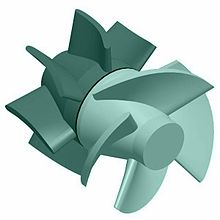
\includegraphics[scale=0.65]{images/fig1.png}
        \legend{Fonte: Wikipédia \cite{wiki_bomba_axial}}
        % \legend{Fonte: Wikipédia \footnote{Bombas Axiais}}
    \end{figure}


    Já o sistema diretor, tem como função, coletar o fluido e dirigi-lo para um caminho determinado. No caso das bombas centrífugas, o sistema diretor de saída é simplesmente um difusor, que transforma parte da energia de velocidade em energia de pressão. Já nas turbinas, o sistema diretor é fundamentalmente um injetor, conforma mostrado na \autoref{fig2:sist_diretor_pelton}, que transforma parte da energia de pressão em energia de velocidade.

    \begin{figure}[htb]
        \centering
        \caption {\label {fig2:sist_diretor_pelton} Sistema diretor de uma turbina hidráulica do tipo Pelton}
        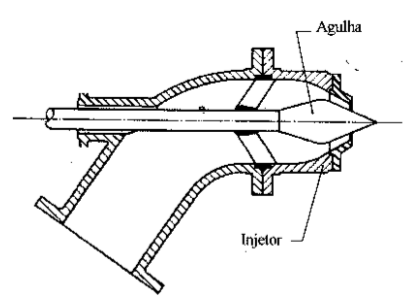
\includegraphics[scale=0.5]{images/fig2.png}
        \legend{Fonte: Máquinas de Fluidos \cite{maq_fluidos_henn}}
    \end{figure}

\subsection{Tipos de Turbinas Hidráulicas}

\subsubsection{Turbina tipo Francis}

A turbina Francis, é uma turbina hidráulica que foi concebida por Jean-Victor Poncelet por volta de 1820 e aperfeiçoado pelo engenheiro norte-americano James B. Francis \cite{turbina_francis}. Ela se comporta com o fluxo radial de fora para dentro, conforme pode ser visto na Figura \ref{fig3:turbina_francis}.

    \begin{figure}[htb]
        \centering
        \caption {\label{fig3:turbina_francis} Ilustração de uma turbina Francis}
        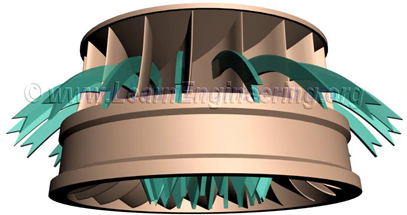
\includegraphics[scale=0.8]{images/fig3.png}
        \legend{Fonte: Learn Engineering \cite{francis_turbine}}
    \end{figure}

    É uma das turbinas mais utilizadas na produção de energia elétrica devido ao seu alto grau de eficiência em um grande ramo de operações. O \textit{head} pode variar de 45 a 400 m, e a vazão de 10 a 700 $m^3/s$. \cite{francis_turbine}

\subsubsection{Turbina tipo Kaplan}

    A turbina Kaplan é uma turbina hidráulica, inventada por Victor Kaplan. Foi uma evolução da turbina Francis para ter um melhor rendimento com quedas menores. Ela foi projetada para operar com quedas até de 60m, normalmente utilizada entre 2 a 25 e com alta vazão, entre 70 a 800 $m^3/s$. A única diferença entre a turbina Kaplan e a Francis, é o rotor. O rotor da Kaplan se assemelha a um propulsor de navio, conforme pode ser visto na  \autoref{fig4:turbina_kaplan}.

    \begin{figure}[htb]
        \centering
        \caption {\label {fig4:turbina_kaplan} Turbina Kaplan depois de 61 anos de uso. }
        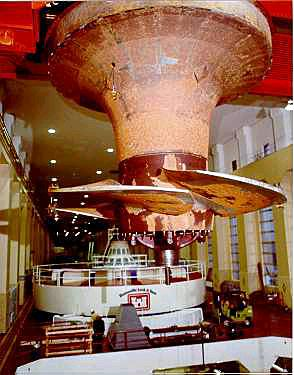
\includegraphics[scale=0.6]{images/fig4.jpg}
        \legend{Fonte: Wikipedia \cite{turbina_kaplan}}
    \end{figure}

\subsubsection{Turbina tipo Pelton}

    \begin{figure}[htb]
        \centering
        \caption {\label{fig5:turbina_pelton} Funcionamento da turbina Pelton}
        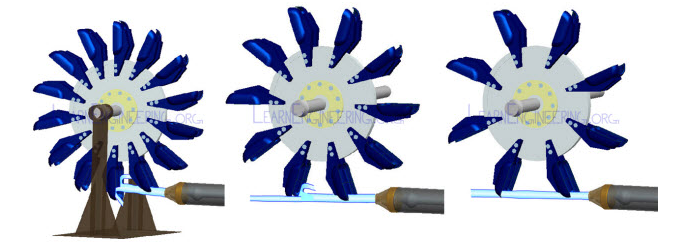
\includegraphics[scale=0.5]{images/fig5.png}
        \legend{Fonte: Learn Engineering \cite{pelton_turbine}.}
    \end{figure}

    Turbina Pelton é uma turbina de ação, isto é, funciona à pressão atmosférica, são adequadas para alto \textit{head}, variando entre 350 $m$ até 1100 $m$ e baixa vazão \cite{pelton_turbine}. Foi inventada por Lester Allan Pelton na década de 1870 \cite{turbina_pelton}.

    É constituída por uma roda, com um ou mais injectores e pás giratórias em forma de dupla concha conforme pode ser visto na \autoref{fig5:turbina_pelton}. Basicamente a turbina Pelton transforma a energia de pressão proveniente do jato de água em alta velocidade em energia de cinética, pois quando o jato incide na dupla concha da turbina Pelton, produz uma força impulsiva que a turbina se movimenta. O eixo rotativo executa um gerador que produz eletricidade.

\subsection{Campo de Aplicação}

    \begin{figure}[htb]
        \centering
        \caption{\label{fig-camp} Campo de aplicação}
        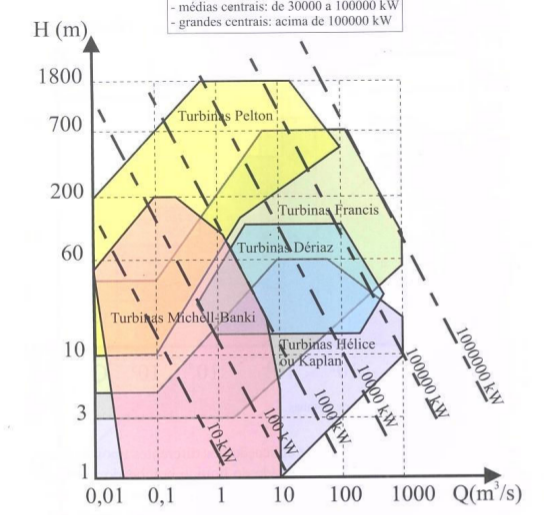
\includegraphics[scale=0.5]{images/campo_de_aplicacao.png}
        \legend{Fonte: Máquinas de Fluidos  \cite{maq_fluidos_henn}.}
    \end{figure}

    Para o ramo das turbinas, existem áreas de superposição entre os campos de aplicação dos diferentes tipos de turbinas, levando em consideração a altura de queda, vazão e a potência. A \autoref{fig-camp} releva predominância em certas áreas de aplicação, como por exemplo de elevada altura de queda e baixa vazão, a turbina Pelton se destaca. Enquanto para grandes vazões e pequena altura de queda a Kaplan se destaca.

\section{Triangulo de Velocidades}

    Um dos conceitos-chave em máquinas de fluxo é entender como o escoamento aparece do ponto de visto do elemento rotativo. Uma vez entendido isso, o entendimento da máquinas de fluxo se torna relativamente mais fácil. Observar a velocidade do escoamento a partir do ponto de vista do rotor em movimento é chamado de \textit{velocidade relativa da corrente fluida} ($\vec{w}$) e a velocidade do escoamento do ponto de vista do observador estacionário é chamado de \textit{velocidade absoluta da corrente fluida} ($\vec{c}$).


    % \begin{figure}[htb]
    %     \centering
    %     \caption {\label{fig7:2motion} Triângulo de velocidades (analogia com o movimento das partículas de água da chuva)}
    %     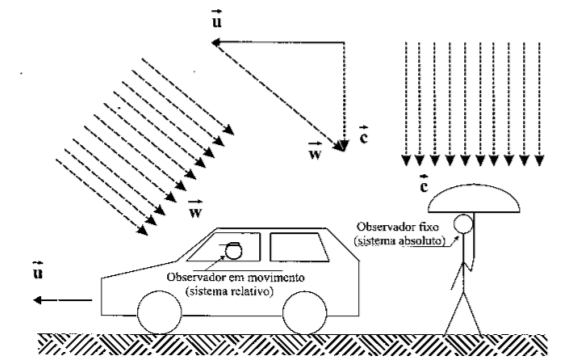
\includegraphics[scale=0.6]{images/fig7.png}
    %     \legend{Fonte: Máquinas de Fluidos  \cite{maq_fluidos_henn}.}
    % \end{figure}
    %
    % Na \autoref{fig7:2motion}, observa-se soma vetorial para o triangulo de velocidades da água da chuva com um carro em movimento, portanto se o observador está em  movimento (como é o caso do elemento rotativo nas máquinas de fluxo), com velocidade $\vec{u}$ e a chuva com a velocidade absoluta da corrente fluida $\vec{c}$, e a soma vetorial dessas velocidades será a velocidade relativa da corrente fluida $\vec{w}$ em relação ao observador em movimento.
    %
    % Nas máquinas de fluxo, o triangulo de velocidades ocorre de forma semelhante conforme demostrado acima. 
    A \autoref{fig8:tri_vel} representa o corte segundo um plano meridiano que passa pelo eixo do rotor e pelo corte segundo um plano perpendicular ao eixo do rotor de uma corrente fluida que circula através do rotor de um ventilador (máquina geradora de fluxo).

    \noindent
    Em um ponto qualquer do rotor, denomina-se: \\
        $\vec{u}$ = \textbf{velocidade tangencial} do referido ponto do rotor; \\
        $\vec{c}$ = \textbf{velocidade absoluta da corrente fluida}; \\
        $\vec{w}$ = \textbf{velocidade relativa da corrente fluida}; \\
        $\alpha$ = ângulo que formam os sentidos positivos de $\vec{u}$ e $\vec{c}$ ; \\
        $\beta$ = ângulo que formam o sentido de $\vec{w}$ com o negativo de $\vec{u}$

    \begin{figure}[htb]
        \centering
        \caption {\label{fig8:tri_vel} Escoamento através do rotor de um ventilador centrífugo (máquina de fluxo geradora)}
        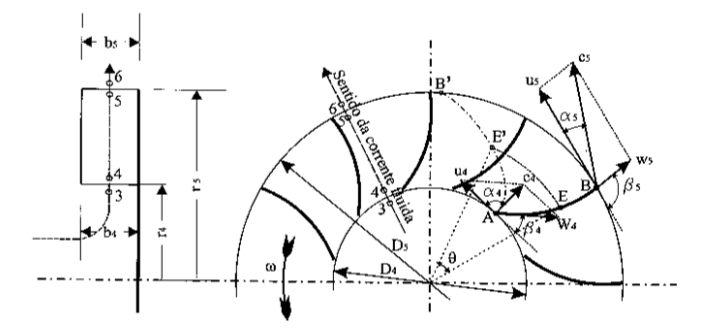
\includegraphics[scale=0.65]{images/fig8.png}
        \legend{Fonte: Máquinas de Fluidos  \cite{maq_fluidos_henn}.}
    \end{figure}

    \noindent
        A estes vetores e suas componentes atribuem-se os seguintes índices: \\
        \textbf{3} = um ponto na corrente de entrada não perturbada, situado imediatamente antes da \textbf{entrada} do rotor; \\
        \textbf{4} = um ponto situado imediatamente depois da entrada do rotor, portanto, já no espaço entre as pás giratórias; \\
        \textbf{5} = um ponto situado imediatamente antes da \textbf{saída} do rotor, portanto, ainda no espaço entre as pás giratórias; \\
        \textbf{6} = um ponto  na corrente de saída não perturbada, situado imediatamente depois da saída do canal móvel.

        Considere a \autoref{fig8:tri_vel} um rotor radial constituído de um número infinito de pás, de espessura infinitesimal, separadas por canais infinitesimais também. Isso implica que o fluxo através dele será unidimensional e que a corrente fluida será tangente às pás do rotor, em todos os seus pontos.

        As pás são construídas de modo inicial para que não haja mudança brusca de direção e perdas de energias devido a formação de vórtices por exemplo. No ponto \textit{A} temos o triângulo de velocidades da corrente fluida imediatamente após a entrada do rotor, e no ponto \textit{B} o triângulo de velocidades da corrente fluida imediatamente antes da saída do rotor. A \autoref{fig9:tri_vel} representa um triângulo de velocidades genérico, em que se faz a decomposição dos vetores $\vec{c}$ e $\vec{w}$ em componentes meridianas com o índice \textit{m} e em componentes tangenciais com o índice \textit{u}.

    \begin{figure}[htb]
        \centering
        \caption {\label {fig9:tri_vel} Triangulo de velocidades genérico }
        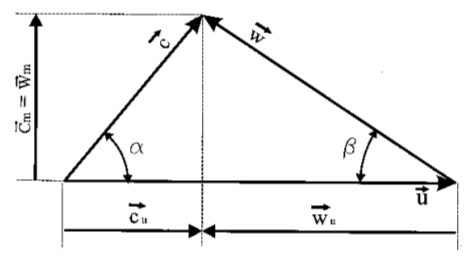
\includegraphics[scale=0.65]{images/fig9.png}
        \legend{Fonte: Máquinas de fluidos  \cite{maq_fluidos_henn}}
    \end{figure}

    A componente tangencial está vinculada com a energia intercambiada entre o rotor e o fluido, enquanto a componente meridiana, de módulo $\vec{c}_m$ está vinculada à vazão da máquina, por meio da equação da continuidade: Q = A $c_m$.

% \section{Máquinas Semelhantes}
%
% \chapter{Motivação}
%
% \section{Exemplos de modelo reduzido}
%
% \section{Projeto}
%
% \chapter{Cálculo e Explicações}

% \chapter*[Considerações Finais]{Considerações Finais}
% \addcontentsline{toc}{chapter}{Considerações Finais}

\section {Números adimensionais}

\subsection{Coeficiente de Reynolds}

    O número de Reynolds é bastante utilizado na mecânica dos fluidos, principalmente para determinar a classificação do escoamento, se é laminar, transiente ou turbulento. Seu significado físico é o quociente de forças de inércia ($V \rho$) entre forças de viscosidade ($\mu/D$), e é expressado como:

    \begin{equation} \label{eq-reynolds}
        Re = \frac{\rho V D}{\mu}
    \end{equation}

    Onde, $\rho$ é a massa específica do fluido, $V$ velocidade do fluido, $D$ o diâmetro da tubulação e $\mu$ a viscosidade cinemática do fluido.

\subsection {Coeficiente de forma}

    A equação abaixo representa a \textbf{velocidade de rotação específica} ou \textbf{coeficiente de forma} do rotor. Ela é adimensional e seu valor numérico mantém constante para máquinas de fluxo semelhantes, independente do sistema de unidades usado no cálculo.
    \begin{equation} \label{eq-na}
        n_{qA} = 10^3 \; . \; n \; . \; \frac{Q^{\rfrac{1}{2}}}{Y^{\rfrac{3}{4}}}
    \end{equation}

\noindent
    Onde:  \\
    $n_{qA} =$ velocidade de rotação específica ou coeficiente de forma do rotor; \\
    $n$ = velocidade de rotação da máquina, em $rps$ (Hz); \\
    $Q$ = vazão da máquina, em $m^3/s$; \\
    $Y$ = salto energético específico, em $J/kg$.

% \indent

    Os valores de $n$, $Q$, e $Y$, utilizados no cálculo do $n_{qA}$ correspondem ao ponto de projeto ou melhor rendimento. Para máquinas de vários estágios (rotores em série) o $Y$ utilizado corresponde ao salto energético específico de cada rotor, e para rotores com dupla sucção, utiliza-se a vazão $Q$ de um dos tubos de sucção.

    \begin{table}[htb]
         \setlength{\tabcolsep}{20pt} % General space between cols (6pt standard)
        \centering
        \caption{Valores de $n_{qA}$ indicados para diferentes tipos de máquinas de fluido.}
        \label{tab-na}
        % \begin{tabular}{p{2.6cm}|p{6.0cm}|p{2.25cm}|p{3.40cm}}
        % \resizebox{0.35\textwidth}{!}{%
        \begin{tabular}{l  l}
            \toprule
            Para turbina hidráulica do tipo Pelton & $n_{qA} =$ 5 a 70 \\
            \hline
            Para turbina hidráulica do tipo Francis lenta & $n_{qA} =$ 50 a 120 \\
            % \hline
            % Para turbina hidráulica do tipo Francis normal & $n_{qA} =$ 120 a 200 \\
            \hline
            Para turbina hidráulica do tipo Francis rápida & $n_{qA} =$ 200 a 320 \\
            \hline
            Para turbina hidráulica do tipo Michel-Banki  & $n_{qA} =$ 30 a 210 \\
            \hline
            Para turbina hidráulica do tipo Dériaz  & $n_{qA} =$ 200 a 450 \\
            \hline
            Para turbina hidráulica do tipo Kaplan e Hélice  & $n_{qA} =$ 300 a 1000 \\
            \hline
            Para turbina a vapor e gás com admissão parcial & $n_{qA} =$ 6 a 30 \\
            \hline
            Para turbina a vapor e gás com admissão total & $n_{qA} =$ 30 a 300 \\
            \hline
            Para bomba de deslocamento positivo & $n_{qA} <$  30 \\
            \hline
            Para bomba centrifuga & $n_{qA} =$  30 a 250 \\
            \hline
            Para compressor de deslocamento positivo & $n_{qA} <$ 20 \\
            \hline
            Para ventilador e turbocompressor centrífugo & $n_{qA} = 20$ a 330 \\
            \hline
            Para ventilador e turbocompressor axial & $n_{qA} =$ 330 a 1800 \\
            \bottomrule
        \end{tabular} %}
        \legend {Fonte: Máquinas de fluidos  \cite{maq_fluidos_henn}}
    \end{table}


\section{Perda de Carga}

    O assunto perda de carga é extenso dentro da mecânica dos fluidos, será tratado aqui apenas o essencial para o desenvolvimento do projeto. Sabe-se que entre dois pontos de um fluido é possível aplicar a equação abaixo, com as seguintes condições: escoamento permamente, incompreensível, completamente desenvolvido, energia interna e pressão uniforme em 1 e 2 \cite{fox}.

    \begin{equation} \label{eq-perda_de_carga}
        h_t = \left( \frac{p_1}{\rho} + \frac{V^2_1}{2} + gz_1 \right)- \left( \frac{p_2}{\rho} + \frac{V^2_2}{2} + gz_2 \right)
    \end{equation}

\noindent
    Onde: \\
    $h_t$ : Perda de carga total da tubulação entre os pontos 1 e 2. \\
    $p$   : Pressão nos pontos 1 e 2. \\
    $\rho$ : Massa específica do fluido. \\
    $z$ : Cota geométrica do ponto 1 e 2. \\
    $V$: Velocidade nos pontos 1 e 2.


    Para um escoamento laminar, é possível calcular a ($h_t$) analiticamente, porém tubulação desenvolvida para o projeto, o escoamento é turbulento e o cálculo da perda de carga ($h_t$) é encontrado por uma fórmula empírica em base dados experimentais, conhecida por Darcy-Weisbach:
    \begin{equation} \label{eq-darcy}
        h_{maior} = f \frac{L}{D} \frac{V^2}{2}
    \end{equation}

    \noindent
    Onde \\
    $f$: fator de atrito \\
    $L$: Comprimento do duto \\
    $D$: Diâmetro interno do duto \\
    $V$: Velocidade no duto

    E $h_{maior}$ é denominado perda de carga maior, pois é onde terá uma maior contribuição para a perda de carga total, as perdas menores são devido uma variedade de acessórios, curvas ou mudanças súbitas de área \cite{fox} que não serão consideradas na tubulação do projeto.

    O fator de atrito $f$ pode ser calculado através da fórmula de Colebrook \cite{fox}, que serve para evitar o uso do Diagrama de Moody nos escoamentos turbulentos:

    \begin{equation} \label{eq-colebrook}
    \frac{1}{f^{0,5}} = -2,0 \log \left( \frac{e/D}{3,7} + \frac{2,51}{Re\;f^{0,5}} \right)
    \end{equation}

    Que é facilmente resolvida dando-lhe um valor inicial arbitrário  e fazendo a iteração dos novos valores, pois converge rapidamente.

\section{Máquinas de fluxo semelhantes}

    Há diversas vantagens em se construir máquinas de fluxo semelhantes, enquanto para modelos reduzidos permite diminuir a execução errônea de máquinas de grande porte, a construção de modelos aumentados muitas vezes se faz necessária para facilitar as medições durante os ensaios \cite{maq_fluidos_henn}.

    Para que duas máquinas sejam consideradas semelhantes, é necessário satisfazer algumas condições, como semelhanças geométricas, cinemáticas e dinâmicas.

    A \textbf{semelhança geométrica} significa que as duas máquinas devem ter as mesmas dimensões lineares, igualdade de ângulos e nenhuma omissão ou adição de partes. Para uma máquina de fluxo modelo (índice ``m'') e máquina protótipo (índice ``p'') sejam semelhantes geometricamente, é necessário que:

    \begin{equation} \label{eq-geometrica}
        \frac{D_{5p}}{D_{5m}} = \frac{b_{5p}}{b_{5m}} = \frac{D_{4p}}{D_{4m}} = k_G = \mbox{constante}
    \end{equation}

    Onde $k_G$ é denominado escala geométrica ou \textbf{fator de escala} e os ângulos de entrada e saída do protótipo e modelo também necessitam ser iguais, logo:

    \begin{equation}
        \beta_{4p} = \beta_{4m} \; \; \; \mbox{e} \; \; \; \beta_{5p} = \beta_{5m}
    \end{equation}

    Já a \textbf{semelhança cinemática} significa que as velocidades e acelerações, para pontos correspondentes, sejam vetores paralelos e possuam relação constante entre seus módulos, ou seja:

    \begin{equation}
    \frac{c_{m4p}}{c_{m4m}} = \frac{c_{u5p}}{c_{u5m}} = \frac{u_{5p}}{u_{5m}} = k_c = \mbox{constante}     \end{equation}

    Onde $k_c$ é denominado \textbf{escala de velocidades}. E a \textbf{semelhança dinâmica} significa que os tipos idênticos de forças sejam vetores paralelos e que a relação entre seus módulos seja constante para pontos correspondentes, ou seja:

    \begin{equation}
        \frac{F_{inércia,p}}{F_{inércia,m}} = \frac{F_{atrito,p}}{F_{atrito,m}} = k_D = \mbox{constante}
    \end{equation}

    Onde $k_D$ é denominada de \textbf{escala dinâmica}.

    É possível testar se duas máquinas realmente são semelhantes se cumprirem-se, simultaneamente, a igualdade do número de reynolds, do número de Mach, do número de Froude, do número Weber e do número de Euler. Contudo, o mais importante é o número de Reynolds para a semelhança dinâmica.

     As grandezas biunitárias são feitas restrições de salto energético específico unitário, diâmetro característico do rotor unitário, semelhança cinemática e rendimento hidráulico constante entre modelo e protótipo, A \textbf{velocidade de rotação biunitária} ($n_{11}$) é dada por:

     \begin{equation} \label{eq-vel-bi}
         n_{11} = \frac{n\: D}{Y^{\rfrac{1}{2}}}
    \end{equation}

    \noindent
    Onde: \\
    $n_{11}$ = velocidade de rotação biunitária, no Sistema Internacional de Unidades, em $kg^{1/2}\: m/J^{1/2}s$; \\
    $n$ = velocidade de rotação da máquina considerada, em rps ou Hz; \\
    $D$ = diâmetro característico do rotor da máquina considerada; \\
    $Y$ = salto energético da máquina considerada, em $J/kg$.

    Outra grandeza biunitária bastante utilizada em máquinas de fluxo, é a \textbf{potência no eixo biunitária} que é dada por:

    \begin{equation} \label{eq-pot-bi}
        P_{e11} = \frac{P_e}{D^2 \: Y^{3/2}}
    \end{equation}



\chapter{Justificativa}
    Construir um modelo reduzido é uma ótima oportunidade para compreender e prever o funcionamento de uma turbina real, já que pode-se testar e verificar o funcionamento no modelo reduzido. Desse modo, é possível reduzir o custo e o trabalho a ser executado de maneira significativa, otimizando o processo e o desenvolvimento da turbina. Caso não se faça isso, seria uma enorme perda de tempo e dinheiro caso fosse construído a turbina em enormes dimensões e para verificar que não produz a potência requerida com seu rendimento.

\chapter{Metodologia} % e as considerações

    O projeto de Escoamento é uma disciplina do curso de Engenharia Mecânica da Universidade Federal do Rio de Janeiro - \textit{campus} Macaé com o intuito de consolidar e concatenar os diferentes conteúdos acadêmicos vistos nas disciplinas de Mecânicas dos Fluidos e Máquinas de Fluxo principalmente. Foi proposto encontro quinzenais com o Prof. Eng. Marcelo Silva para a orientação deste trabalho, as principais fontes de consulta foram os livros de Máquinas de Fluidos do autor Érico A. L. Henn \cite{maq_fluidos_henn} e Introdução a Mecânica dos Fluidos de Ronald W. Fox,  \textit{et al} \cite{fox}, e Fluid Mechanics de Frank White \cite{white}.

    Para a realização do projeto, foi dividido em três partes: a primeira – que engloba a determinação de qual turbina operará através do cálculo do coeficiente de forma, assim como a velocidade do jato d'água na saída da tubulação. Nessa parte, a avaliação da perda de carga na tubulação assim como as simplificações feitas foram cruciais para a realização do projeto, a segunda - que apresenta os cálculos realizados na turbina real para os dados fornecidos e resultados anteriores, e a terceira - que engloba toda análise feita no modelo reduzido à partir das informações anteriores.

% comé que começou o trabalho, como o grupo começou a reunir, as principais fonte de consulta, a principio começou em livro e tivemos encontros quinzemais com o prof. eng. marcelo silva, dividomos o trabalho em etapa, consultas bibliograficas, na terceira etapa escrever trab

    % Os critérios a serem analisados são: aplicação dos métodos estatísticos estudados na disciplina; justificativa das conclusões tiradas e decisões tomadas, à luz dos métodos estatísticos estudados; capacidade crítica revelada pelo grupo em relação aos resultados; apresentação e qualidade do texto.

\chapter{Calculos}

     Relembrando, deseja-se uma turbina hidráulica que possui as seguintes características: operando em água, de massa específica ($\rho$) de $1000\;kg/m^3$, altura de queda ($H$) de 342 m, vazão ($Q$) de $2,23\;m^3/s$ e velocidade de rotação ($n$) de $300\;rpm$.

    \noindent
    \textbf{Dados adicionais}: \\
    Diâmetro do injetor ($D_i$): 0,20 $m$. \\
    Diâmetro da tubulação ($D_t$): 0,750 $m$. \\
    Viscosidade cinemática da água ($\mu$): $1,00 \times 10^{-3}\; Pa\:.\:s$. \\
    Comprimento da tubulação ($L$): 1000 $m$ \\
    Rugosidade da tubulação ($e$): 0,00026 $m$


\section{Seleção do tipo de Turbina}

    Para a turbina com dimensões reais serão identificadas pelo subscrito ``p'', enquanto para a turbina modelo serão pelo subscrito ``m''. Para selecionar o tipo de turbina que operará com essas condições, deve-se calcular o coeficiente de forma do rotor $n_{qA}$ e verificar na \autoref{tab-na} a máquina que possui o melhor rendimento.


    Primeiro, transforma a velocidade de rotação ($n_p$) que está rotações por minuto para rotações por segundo, dividindo por 60, tem-se $n_p = 5\;rps$, para a unidade da equação \eqref{eq-na} ser coerente e ter o coeficiente na forma adimensional.
    A energia por unidade de massa que o fluido entrega para a máquina será $ Y_p = g \; H_p = 9,81 \; . \; 342 = 3\;335,02\;J/kg $. Aplicando a equação \eqref{eq-na}, resulta em:
    \begin{equation*}
        n_{qA} = 10^3 \; . \; 5 \; . \; \frac{2,23^{0,5}}{3\;355,02^{0,75}} = 16,94
    \end{equation*}

    Que se enquadra na máquina de melhor rendimento a turbina Pelton visto na \autoref{tab-na}, e reforçado pela \autoref{fig-camp}.


\section{Velocidade do jato d'água ($V_j$) na saída do injetor}

    \begin{figure}[htb]
        \centering
        \caption{ \label{fig-pelton} Representação esquemática da turbina Pelton.}
        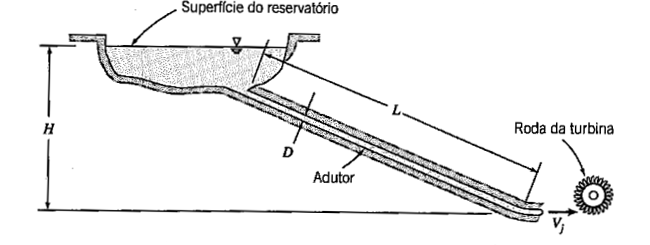
\includegraphics[scale=0.6]{images/turbina_pelton_fox.png}
        \legend{Fonte: Introdução a Mecânica dos Fluidos \cite{fox}}
    \end{figure}

    A \autoref{fig-pelton} representa um esquema da turbina pelton. Aplicando a equação \eqref{eq-perda_de_carga} de perda de carga total que será igual a equação de perda maior \eqref{eq-darcy},e considerando para um escoamento permanente, incompressível, completamente desenvolvido, no nível montante (1) e na saída do injetor (j), resulta em:
    \begin{equation*}
        \bigg( \cancel{\frac{p_1}{\rho}} + \cancelto{0}{\frac{V^2_1}{2}} + gz_1 \bigg) - \left( \cancel{\frac{p_j}{\rho}} + \frac{V^2_j}{2} + \cancelto{0}{gz_j} \;\;\: \right) = h_t = f \frac{L}{D}\: \frac{V_t^2}{2}
    \end{equation*}

    Como $p_1$ = $p_j$ = pressão atmosférica, e considerando o nível constante em 1 ($V_1 = 0$), e o nível de referência adotado na saída do injetor ($z_j$ = 0). Substituindo $z_1$ por $H$, é possível reorganizar a equação de cima para $V_j$:

    \begin{equation*}
        V_j^2 = 2gH - f \frac{L}{D} V_t^2
    \end{equation*}

    Em que $V_t$ é a velocidade do fluido dentro da tubulação e $V_j$ a velocidade do jato na saída do injetor. A velocidade do jato e a velocidade do tubo estão relacionados pela equação da continuidade: $A_t\: V_t = A_i \: V_j$. Assim, $V_t =  \frac{A_i}{A_t} \: V_j$ = $\left(\frac{D_i}{D_t} \right)^2 \: V_j$. Substituindo na equação de cima e reorganizando novamente para $V_j$, resulta em:

    \begin{equation} \label{eq-jato}
        V_j = \left[ \cfrac{2gH}{\left\{1 + f\cfrac{L}{D_t} \left(\cfrac{D_i}{D_t} \right)^4 \right\}} \right]^{\frac{1}{2}}
    \end{equation}

    A equação \eqref{eq-jato} fornece a velocidade do jato na saída do injetor já com a correção das perdas de carga na tubulação de adução, pois a perda de carga depende do comprimento da tubulação ($L$), o diâmetro da tubulação ($D_t$), o diâmetro interno do injetor ($D_i$) e altura de queda ($H$) e o fator de atrito $f$.

    Para calcular o fator de atrito $f$ foi utilizado a equação \eqref{eq-colebrook} de Colebrook, no entanto esta equação depende da rugosidade relativa e do número de Reynolds, e o número de Reynolds depende da velocidade da tubulação ($V_t$), mas não temos essa velocidade.

    Para resolver esse problema, foi proposto uma resolução através iteração, primeiro atribuiu-se um valor para a velocidade do jato sem a perda de carga, que é igual à $V_{j,i} = \sqrt{(2gH)} = 81,91 m/s$. Com esta velocidade inicial, podemos determinar a velocidade da tubulação $V_t$ através da equação da continuidade, logo em seguida calcula-se o número de Reynolds com a equação \eqref{eq-reynolds} para determinar o fator de atrito com a equação \eqref{eq-darcy} e logo em seguida aplica a equação \eqref{eq-jato} para determinar a nova velocidade do jato e repetir todo o processo, conforme está ilustrado no fluxograma à seguir:

    \begin{figure}[htb]
        \centering
        \caption{\label{fig-fluxo} Fluxograma representando o processo iterativo}
        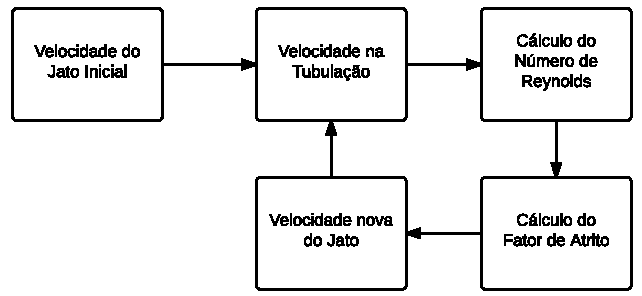
\includegraphics[scale=1]{images/fluxograma.pdf}
        \legend{Fonte: Figura elaborada pelos autores.}
    \end{figure}

    % \lstinputlisting[language=Python]{iteracao.py}

    % \begin{equation*}
    %
    % \end{equation*}

    Para executar o fluxograma da \autoref{fig-fluxo}, foi realizado pelos autores um programa computacional na linguagem de programação Python que se encontra no \autoref{ap-python}. O resultado da velocidade de saída do jato d'água $(V_j$) para uma tubulação feita de ferro fundido, e portanto, rugosidade ($e$) de 0,00026 $m$, convergiu para: $\mathbf{78,31\:} m/s$.

    \section{A velocidade absoluta do fluido $V_{j,c}$ na entrada do rotor}

    \begin{figure}[htb]
        \centering
        \caption{\label{fig-pelton_white} Velocidade do fluido na entrada do rotor}
        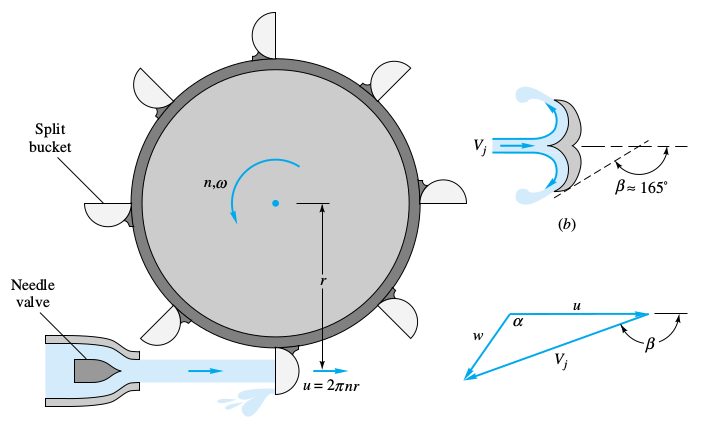
\includegraphics[scale=0.5]{images/pelton_turbine.png}
        \legend{Fonte: Fluid Mechanics \cite{white}.}
    \end{figure}
    A \autoref{fig-pelton_white} representa o funcionamento da turbina Pelton proveniente do jato d'água e demostra o triângulo de velocidades fornecido para um ângulo arbitrário $\beta$.

    Para um bocal perfeito, a velocidade do jato sem a perda de atrito seria a velocidade $V_j = 78,31 \: m/s$, no entanto considerando o bocal com superfícies irregulares, então a velocidade do jato corrigida será $V_{j,c} =  C_v \: V_{j}$, onde o coeficiente de velocidade ($C_v$) é usado e varia entre $0,92 \leq C_v \leq 0,98$. Considerando uma condição típica de trabalho, que é de um ângulo ($\beta$) de $160^{\circ}$, e $C_v$ igual à 0,94, ou seja, uma perda de 6\% segundo Frank White \cite{white}. Portanto a velocidade do jato d'água corrigida ($V_{j,c}$) é de  $73,61\: m/s$.

\section{Diâmetro do rotor da turbina modelo}

    \begin{figure}[htb]
        \centering
        \caption{\label{fig-rendimento} Eficiência de uma turbina de ação}
        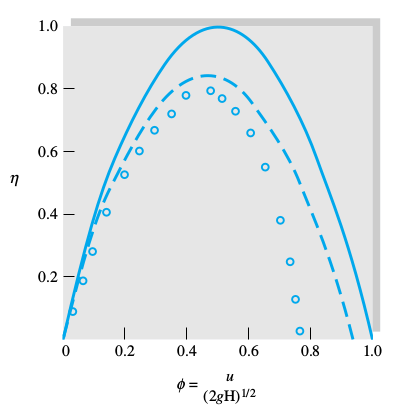
\includegraphics[scale=0.5]{images/eficiencia_pelton.png}
        \legend{Fonte: Fluids Mechanics \cite{white}.}
    \end{figure}

    A \autoref{fig-rendimento} representa a eficiência ($\eta$) de uma turbina de ação, como é a turbina Pelton para diferentes valores da relação da velocidade absoluta do rotor ($u$), com a velocidade absoluta do jato d'água sem a correção $V_j$, para essas condições de trabalho o máximo rendimento é ($\eta_{max}$) = 85\%, e $\phi$ é igual à 0,47 \cite{white}.

    Sendo assim, a velocidade absoluta do rotor será:
    \begin{equation*}
        u = 0,47 \; . \; V_{j,c} = 0,47 \; . \; 73,61 = 34,60 \: m/s
    \end{equation*}

    O diâmetro do rotor do protótipo pode então ser calculado através da equação básica da velocidade angular $u = 2 \pi r n = \pi D n$ e rearranjando para o diâmetro, tem-se:

    \begin{equation*}
        D_p = \frac{u}{\pi \; . \; 5} = 2,20\: m
    \end{equation*}

    Como o fator de escala é $k_G = \frac{D_p}{D_m} = 10$, o diâmetro do rotor no modelo é, utilizando a equação \eqref{eq-geometrica}:

    \begin{equation*}
        D_m = \frac{D_p}{k_G} = \frac{2,20}{10} = 0,220\:m \mbox{ ou } 220\: mm
    \end{equation*}

\section{A velocidade de rotação da turbina modelo}

    A altura de queda também será de 10 (dez) vezes menor, desse modo:
    \begin{equation*}
        H_m = \frac{H_p}{10} = \frac{342}{10} = 34,2\:m \implies Y_m = g \: . \: H_m = 9,81 \: . \: 34,2 = 335,5\: J/kg
    \end{equation*}

    Como as grandezas biunitárias são iguais para máquinas de fluxo semelhantes, com base na equação \eqref{eq-vel-bi} pode-se escrever:
    \begin{equation*}
        \begin{split}
            n_{11} &= \frac{n_m \: D_m}{Y_m^{\rfrac{1}{2}}} = \frac{n_p \: D_p}{Y_p^{\rfrac{1}{2}}} \; \therefore \\
            n_m &= n_p \: \frac{D_p}{D_m}\: \left(\frac{Y_m}{Y_p} \right)^{\rfrac{1}{2}} = 5\; \frac{2,20}{0,220} \left( \frac{335,5}{3355,02} \right)^{\rfrac{1}{2}} \; \therefore \\
            n_m &= 15,81 \: rps \mbox{ ou } 948,68\: rpm
        \end{split}
    \end{equation*}

\section{A potência no eixo da turbina modelo}

    Considerando as perdas na instalações ignoradas e um rendimento de, $\eta_p = 0,85$, a potência do protótipo pode ser calculada pela equação abaixo:
    \begin{equation*}
        P_{ep} = \rho \, . \, Q_p \, . \, Y_p \, . \, \eta_p = 1000 \, . \, 2,23 \, . \, 3355,02 \, . \, 0,85 = 6359,4 \: \mbox{kW}
    \end{equation*}

    E considerando um rendimento invariável entre modelo e protótipo, o modelo também operando com água, a equação \eqref{eq-pot-bi} permite estabelecer:
    \begin{equation*}
        \begin{split}
            P_{e11} &= \frac{P_{em}}{D_m^2 \: . \: Y_m^{\rfrac{3}{2}}} = \frac{P_{ep}}{D_p^2 \: . \: Y_p^{\rfrac{3}{2}}} \; \therefore \; P_{em} = P_{ep} \; \left( \frac{D_m}{D_p} \right)^2 \left( \frac{Y_m}{Y_p} \right)^{ \! \rfrac{3}{2}} \; \therefore  \\
            P_{em} &= 6359,4 \left( \frac{0,220}{2,20} \right)^2 \left( \frac{335,5}{3355,02} \right)^{\rfrac{3}{2}} = 2,01 \; \mbox{kW} 
        \end{split}
    \end{equation*}

% \chapter*[Considerações Finais]{Considerações Finais}
% \addcontentsline{toc}{chapter}{Considerações Finais}
\chapter{Considerações Finais}

    A proposta da disciplina que foi consolidar e concatenar as disciplinas da área de escoamento foi atingida no momento em que foi observado a necessidade de ter aprendido cada conteúdo para a realização deste projeto, além da elaboração de um trabalho acadêmico nas normas da ABNT.

    No projeto, muitas simplificações foram feitas assim como alguns itens foram cortados, como a perda de carga localizada de acessórios, perdas por atrito do jato d'água com as paredes das pás, perdas internas da turbina ignoradas, entre outras, é possível fazer uma análise mais abrangente considerando essas perdas. Depois de obtido os dados da turbina no modelo reduzido através dos cálculos, seria possível construir o modelo e começar os testes para a análise da turbina e modificação para que quando construir o protótipo, não tenha surpresas.

% 
     Relembrando, deseja-se uma turbina hidráulica que possui as seguintes características: operando em água, de massa específica ($\rho$) de $1000\;kg/m^3$, altura de queda ($H$) de 342 m, vazão ($Q$) de $2,23\;m^3/s$ e velocidade de rotação ($n$) de $300\;rpm$.

    \noindent
    \textbf{Dados adicionais}: \\
    Diâmetro do injetor ($D_i$): 0,20 $m$. \\
    Diâmetro da tubulação ($D_t$): 0,750 $m$. \\
    Viscosidade cinemática da água ($\mu$): $1,00 \times 10^{-3}\; Pa\:.\:s$. \\
    Comprimento da tubulação ($L$): 1000 $m$ \\
    Rugosidade da tubulação ($e$): 0,00026 $m$


\section{Seleção do tipo de Turbina}

    Para a turbina com dimensões reais serão identificadas pelo subscrito ``p'', enquanto para a turbina modelo serão pelo subscrito ``m''. Para selecionar o tipo de turbina que operará com essas condições, deve-se calcular o coeficiente de forma do rotor $n_{qA}$ e verificar na \autoref{tab-na} a máquina que possui o melhor rendimento.


    Primeiro, transforma a velocidade de rotação ($n_p$) que está rotações por minuto para rotações por segundo, dividindo por 60, tem-se $n_p = 5\;rps$, para a unidade da equação \eqref{eq-na} ser coerente e ter o coeficiente na forma adimensional.
    A energia por unidade de massa que o fluido entrega para a máquina será $ Y_p = g \; H_p = 9,81 \; . \; 342 = 3\;335,02\;J/kg $. Aplicando a equação \eqref{eq-na}, resulta em:
    \begin{equation*}
        n_{qA} = 10^3 \; . \; 5 \; . \; \frac{2,23^{0,5}}{3\;355,02^{0,75}} = 16,94
    \end{equation*}

    Que se enquadra na máquina de melhor rendimento a turbina Pelton visto na \autoref{tab-na}, e reforçado pela \autoref{fig-camp}.


\section{Velocidade do jato d'água ($V_j$) na saída do injetor}

    \begin{figure}[htb]
        \centering
        \caption{ \label{fig-pelton} Representação esquemática da turbina Pelton.}
        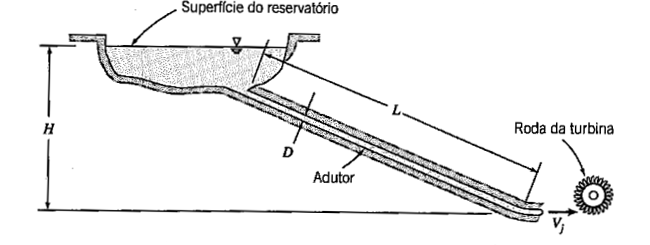
\includegraphics[scale=0.6]{images/turbina_pelton_fox.png}
        \legend{Fonte: Introdução a Mecânica dos Fluidos \cite{fox}}
    \end{figure}

    A \autoref{fig-pelton} representa um esquema da turbina pelton. Aplicando a equação \eqref{eq-perda_de_carga} de perda de carga total que será igual a equação de perda maior \eqref{eq-darcy},e considerando para um escoamento permanente, incompressível, completamente desenvolvido, no nível montante (1) e na saída do injetor (j), resulta em:
    \begin{equation*}
        \bigg( \cancel{\frac{p_1}{\rho}} + \cancelto{0}{\frac{V^2_1}{2}} + gz_1 \bigg) - \left( \cancel{\frac{p_j}{\rho}} + \frac{V^2_j}{2} + \cancelto{0}{gz_j} \;\;\: \right) = h_t = f \frac{L}{D}\: \frac{V_t^2}{2}
    \end{equation*}

    Como $p_1$ = $p_j$ = pressão atmosférica, e considerando o nível constante em 1 ($V_1 = 0$), e o nível de referência adotado na saída do injetor ($z_j$ = 0). Substituindo $z_1$ por $H$, é possível reorganizar a equação de cima para $V_j$:

    \begin{equation*}
        V_j^2 = 2gH - f \frac{L}{D} V_t^2
    \end{equation*}

    Em que $V_t$ é a velocidade do fluido dentro da tubulação e $V_j$ a velocidade do jato na saída do injetor. A velocidade do jato e a velocidade do tubo estão relacionados pela equação da continuidade: $A_t\: V_t = A_i \: V_j$. Assim, $V_t =  \frac{A_i}{A_t} \: V_j$ = $\left(\frac{D_i}{D_t} \right)^2 \: V_j$. Substituindo na equação de cima e reorganizando novamente para $V_j$, resulta em:

    \begin{equation} \label{eq-jato}
        V_j = \left[ \cfrac{2gH}{\left\{1 + f\cfrac{L}{D_t} \left(\cfrac{D_i}{D_t} \right)^4 \right\}} \right]^{\frac{1}{2}}
    \end{equation}

    A equação \eqref{eq-jato} fornece a velocidade do jato na saída do injetor já com a correção das perdas de carga na tubulação de adução, pois a perda de carga depende do comprimento da tubulação ($L$), o diâmetro da tubulação ($D_t$), o diâmetro interno do injetor ($D_i$) e altura de queda ($H$) e o fator de atrito $f$.

    Para calcular o fator de atrito $f$ foi utilizado a equação \eqref{eq-colebrook} de Colebrook, no entanto esta equação depende da rugosidade relativa e do número de Reynolds, e o número de Reynolds depende da velocidade da tubulação ($V_t$), mas não temos essa velocidade.

    Para resolver esse problema, foi proposto uma resolução através iteração, primeiro atribuiu-se um valor para a velocidade do jato sem a perda de carga, que é igual à $V_{j,i} = \sqrt{(2gH)} = 81,91 m/s$. Com esta velocidade inicial, podemos determinar a velocidade da tubulação $V_t$ através da equação da continuidade, logo em seguida calcula-se o número de Reynolds com a equação \eqref{eq-reynolds} para determinar o fator de atrito com a equação \eqref{eq-darcy} e logo em seguida aplica a equação \eqref{eq-jato} para determinar a nova velocidade do jato e repetir todo o processo, conforme está ilustrado no fluxograma à seguir:

    \begin{figure}[htb]
        \centering
        \caption{\label{fig-fluxo} Fluxograma representando o processo iterativo}
        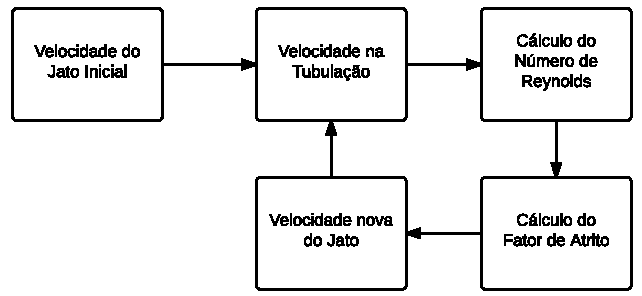
\includegraphics[scale=1]{images/fluxograma.pdf}
        \legend{Fonte: Figura elaborada pelos autores.}
    \end{figure}

    % \lstinputlisting[language=Python]{iteracao.py}

    % \begin{equation*}
    %
    % \end{equation*}

    Para executar o fluxograma da \autoref{fig-fluxo}, foi realizado pelos autores um programa computacional na linguagem de programação Python que se encontra no \autoref{ap-python}. O resultado da velocidade de saída do jato d'água $(V_j$) para uma tubulação feita de ferro fundido, e portanto, rugosidade ($e$) de 0,00026 $m$, convergiu para: $\mathbf{78,31\:} m/s$.

    \section{A velocidade absoluta do fluido $V_{j,c}$ na entrada do rotor}

    \begin{figure}[htb]
        \centering
        \caption{\label{fig-pelton_white} Velocidade do fluido na entrada do rotor}
        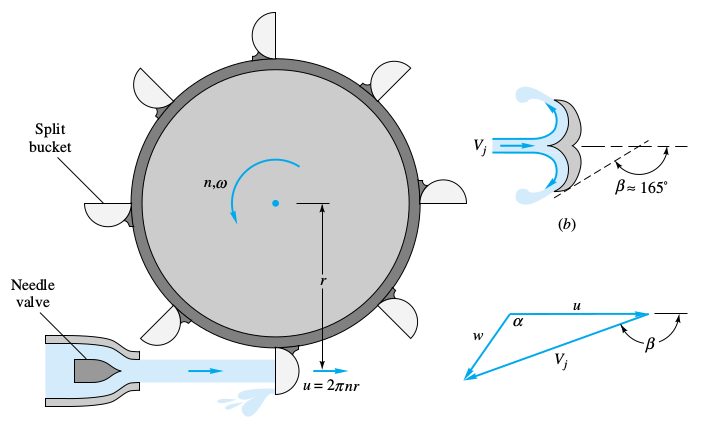
\includegraphics[scale=0.5]{images/pelton_turbine.png}
        \legend{Fonte: Fluid Mechanics \cite{white}.}
    \end{figure}
    A \autoref{fig-pelton_white} representa o funcionamento da turbina Pelton proveniente do jato d'água e demostra o triângulo de velocidades fornecido para um ângulo arbitrário $\beta$.

    Para um bocal perfeito, a velocidade do jato sem a perda de atrito seria a velocidade $V_j = 78,31 \: m/s$, no entanto considerando o bocal com superfícies irregulares, então a velocidade do jato corrigida será $V_{j,c} =  C_v \: V_{j}$, onde o coeficiente de velocidade ($C_v$) é usado e varia entre $0,92 \leq C_v \leq 0,98$. Considerando uma condição típica de trabalho, que é de um ângulo ($\beta$) de $160^{\circ}$, e $C_v$ igual à 0,94, ou seja, uma perda de 6\% segundo Frank White \cite{white}. Portanto a velocidade do jato d'água corrigida ($V_{j,c}$) é de  $73,61\: m/s$.

\section{Diâmetro do rotor da turbina modelo}

    \begin{figure}[htb]
        \centering
        \caption{\label{fig-rendimento} Eficiência de uma turbina de ação}
        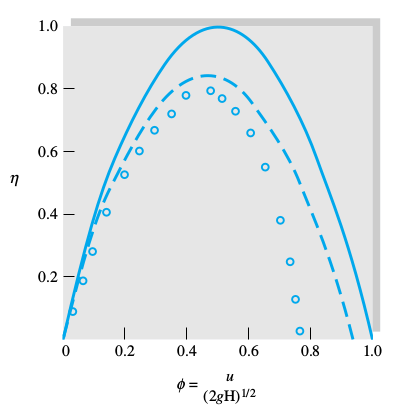
\includegraphics[scale=0.5]{images/eficiencia_pelton.png}
        \legend{Fonte: Fluids Mechanics \cite{white}.}
    \end{figure}

    A \autoref{fig-rendimento} representa a eficiência ($\eta$) de uma turbina de ação, como é a turbina Pelton para diferentes valores da relação da velocidade absoluta do rotor ($u$), com a velocidade absoluta do jato d'água sem a correção $V_j$, para essas condições de trabalho o máximo rendimento é ($\eta_{max}$) = 85\%, e $\phi$ é igual à 0,47 \cite{white}.

    Sendo assim, a velocidade absoluta do rotor será:
    \begin{equation*}
        u = 0,47 \; . \; V_{j,c} = 0,47 \; . \; 73,61 = 34,60 \: m/s
    \end{equation*}

    O diâmetro do rotor do protótipo pode então ser calculado através da equação básica da velocidade angular $u = 2 \pi r n = \pi D n$ e rearranjando para o diâmetro, tem-se:

    \begin{equation*}
        D_p = \frac{u}{\pi \; . \; 5} = 2,20\: m
    \end{equation*}

    Como o fator de escala é $k_G = \frac{D_p}{D_m} = 10$, o diâmetro do rotor no modelo é, utilizando a equação \eqref{eq-geometrica}:

    \begin{equation*}
        D_m = \frac{D_p}{k_G} = \frac{2,20}{10} = 0,220\:m \mbox{ ou } 220\: mm
    \end{equation*}

\section{A velocidade de rotação da turbina modelo}

    A altura de queda também será de 10 (dez) vezes menor, desse modo:
    \begin{equation*}
        H_m = \frac{H_p}{10} = \frac{342}{10} = 34,2\:m \implies Y_m = g \: . \: H_m = 9,81 \: . \: 34,2 = 335,5\: J/kg
    \end{equation*}

    Como as grandezas biunitárias são iguais para máquinas de fluxo semelhantes, com base na equação \eqref{eq-vel-bi} pode-se escrever:
    \begin{equation*}
        \begin{split}
            n_{11} &= \frac{n_m \: D_m}{Y_m^{\rfrac{1}{2}}} = \frac{n_p \: D_p}{Y_p^{\rfrac{1}{2}}} \; \therefore \\
            n_m &= n_p \: \frac{D_p}{D_m}\: \left(\frac{Y_m}{Y_p} \right)^{\rfrac{1}{2}} = 5\; \frac{2,20}{0,220} \left( \frac{335,5}{3355,02} \right)^{\rfrac{1}{2}} \; \therefore \\
            n_m &= 15,81 \: rps \mbox{ ou } 948,68\: rpm
        \end{split}
    \end{equation*}

\section{A potência no eixo da turbina modelo}

    Considerando as perdas na instalações ignoradas e um rendimento de, $\eta_p = 0,85$, a potência do protótipo pode ser calculada pela equação abaixo:
    \begin{equation*}
        P_{ep} = \rho \, . \, Q_p \, . \, Y_p \, . \, \eta_p = 1000 \, . \, 2,23 \, . \, 3355,02 \, . \, 0,85 = 6359,4 \: \mbox{kW}
    \end{equation*}

    E considerando um rendimento invariável entre modelo e protótipo, o modelo também operando com água, a equação \eqref{eq-pot-bi} permite estabelecer:
    \begin{equation*}
        \begin{split}
            P_{e11} &= \frac{P_{em}}{D_m^2 \: . \: Y_m^{\rfrac{3}{2}}} = \frac{P_{ep}}{D_p^2 \: . \: Y_p^{\rfrac{3}{2}}} \; \therefore \; P_{em} = P_{ep} \; \left( \frac{D_m}{D_p} \right)^2 \left( \frac{Y_m}{Y_p} \right)^{ \! \rfrac{3}{2}} \; \therefore  \\
            P_{em} &= 6359,4 \left( \frac{0,220}{2,20} \right)^2 \left( \frac{335,5}{3355,02} \right)^{\rfrac{3}{2}} = 2,01 \; \mbox{kW} 
        \end{split}
    \end{equation*}


\bibliography{bibliografia}

\begin{apendicesenv}

% % Imprime uma página indicando o início dos apêndices
% \partapendices

% ----------------------------------------------------------
\chapter{Programa para determinar a velocidade do jato d'água em Python}
% ----------------------------------------------------------
\label{ap-python}
 \lstinputlisting[language=Python]{iteracao.py}


\end{apendicesenv}
\end{document}
